
\section{Krzysztof Nikodem}
\begin{table}[!h]
\def\arraystretch{2}
\centering
\begin{tabular}{|ll|}
\hline
\multicolumn{2}{|l|}{Optyka}  \\ \hline
\multicolumn{1}{|l|}{kąt graniczny} & $sin \alpha_g_r=\frac{1}{n}$  \\ \hline
\multicolumn{1}{|l|}{kąt Brewstera} & $tg \alpha_B=n$ \\ \hline
\multicolumn{1}{|l|}{zwierciadło kuliste} & $f=\frac{R}{2}$ \\ \hline
\end{tabular}
\caption{Wzory optyka}
\label{optyka}
\end{table}
Pamiętaj o wzorech z tabeli \ref{optyka} ! \\

\textbf{Równanie soczewki} jest równaniniem określającym zależność pomiędzy odległością przedmiotu od soczewki a odległością jego obrazu otrzymanego w tej soczewce.\\

\emph{Równanie soczewki:}
\begin{equation}\label{eq1}
\ \frac{1}{f}=\frac{1}{x}+\frac{1}{y}=(\frac{n_1}{n_2}-1)(\frac{1}{x_1}+\frac{1}{y_1})\\   
\end{equation}
gdzie:
\begin{itemize}
    \item $f$ - odległość ogniskowej od soczewki
    \item $x$ - odległość przedmiotu od soczewki
    \item $y$ - odległość obrazu od soczewki
    \item $r_1,r_2$ - promienie powierzchni kulistych soczewki
    \item $n_1$ - współczynnik załamania ośrodka, w którym znajduje soczewka
    \item $n_2$ - współczynnik załamania soczewki 
\end{itemize}

Każda soczewka posiada oś optyczną i punkt zwany ogniskową. \textbf{Soczewki}  są ograniczone przez powierzchnie kuliste będące wycinkami kul, środki tych kul wyznaczają prostą która jest osią optyczną soczewki. Ogniskowa soczewki jest punktem oznaczanym literą F, który leży na osi optycznej soczewki, w tym punkcie przecinają się kierunki fal lub ich przedłużenia.\\

Soczewki można podzielić w zależności od konstrukcji na soczewki pojedyncze \emph{jak szkło w okularach} i złożone \emph{jak soczewka Fresnela wykorzystywana w latarniach morskich}. Najbardziej rozpowszechnionym podziałem soczewek jest ich podział ze względu na kształt i tu można wyróżnić soczewki przedstawione na: Figure \ref{fig2}.\\

\begin{enumerate}
    \centering
    \item  \emph{dwuwypukłe}
    \item  \emph{płasko-wypukłe}
    \item  \emph{wklęsło-wypukłe}
    \item  \emph{płasko-wklęsłe}
    \item  \emph{dwuwklęsłe}
    
\end{enumerate}

\begin{figure}[]
    \centering
    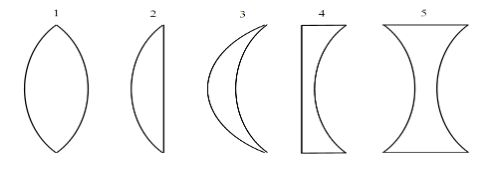
\includegraphics[0.3\textwidth]{pictures/socz.jpg}
    \caption{\emph{Rodzaje soczewek}}
    \label{fig2}
\end{figure}




